\documentclass[11pt]{article}
\usepackage[margin=0.8in]{geometry}
\usepackage{graphicx}
\usepackage{hyperref}
\title{Six-class GLV rho assessment}
\date{2026-10-24}
\begin{document}
\maketitle
\section*{Question and method}
We assessed the six-class GLV walk from Curve Smash commit
\href{https://github.com/Layr-Labs/curvesma.sh/commit/1f084c1914c81a0cdc830b176453adba5dc19ab9}{1f084c1}
against our native default on registered curve \texttt{glv-j0-26}. Its class representative
minimizes the three $x$ rotations and the sign of $y$. The orientation twists the
jump, and distinguished point records carry canonical coefficients.
\begin{center}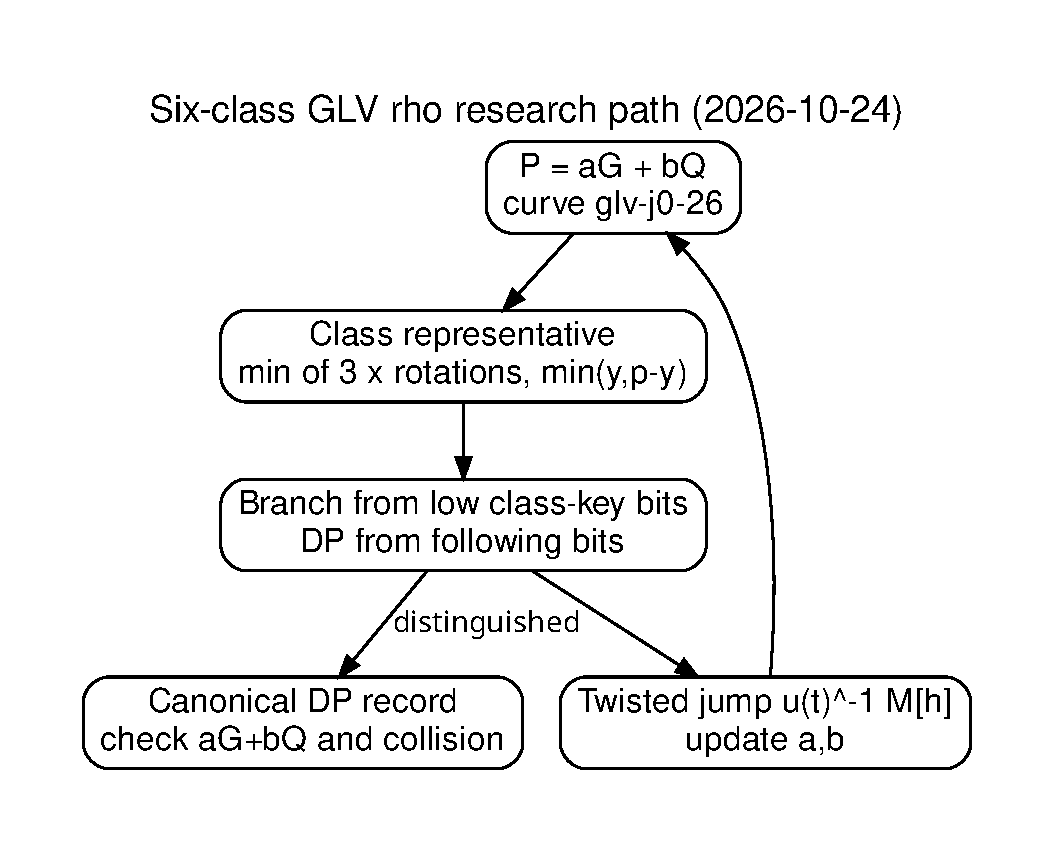
\includegraphics[height=.42\textheight,keepaspectratio]{walk.pdf}\end{center}
\section*{Measured result}
In one paired local run, both solvers recovered all 20 planted logs. Default
oriented GLV rho took 0.016382582 s; six-class DP rho took 0.020590401 s,
1.257 times as long. The candidate visited 46,882 classes, emitted 2,922 DPs,
and took 196 short-cycle escapes. These are total times, with no uncertainty
estimate from this single run.
\begin{center}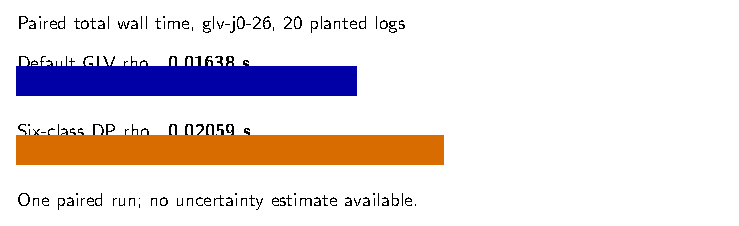
\includegraphics[width=.95\linewidth]{timing.pdf}\end{center}
\section*{Interpretation and limits}
This is a negative toy-curve result. It is not a secp256k1 cost measurement.
Commit 1f084c1 changes $\kappa$ from 1.05 to 1.02 and the inversion batch to
$2^{16}$ while leaving the algorithm unchanged. Its 126.96-bit cost and
$\geq0.3909$ success remain conditional on the stated H1 mixing and cost model.
The C solver is opt-in. A Rust BigUint worker, harness launcher and native Cairn
DP checker provide an end-to-end research path. The C and Rust job derivations
are different, so their receipts cannot be pooled. DP point equations do not
prove walker provenance; sampled re-walks are still required.
\section*{Evidence and next checks}
The source record is \texttt{assessment.md}; raw receipt is
\texttt{paired-glv-j0-26.json}. Repeat paired A/A and A/B tests over the curve
ladder, audit sampled trails, then assess a fixed-limb implementation. No
isogeny-route or volcano graph update follows from this walk.
\end{document}
